\scanpage{59}
\mspage{17}
cas particulier, en faisant $i=j$.

À vrai dire, je vois maintenant que ces fameuses pierres telles quelles sont des côtes mal taillées — ils sont trop \unsure{généraux|généreux}, ou pas assez. Pas assez pour contenir les morceaux $\unsure{\mathcal V|\dot{\mathcal V}}_{d_*,d''_*}^{d'_*}\approxeq\unsure{\check N|\widetilde N}_{d_*;(d'_0,d''_0)}\mid D_{d_*}^*$ de ($\mathrm{Str}_\infty$ p. 84) — trop en ce sens, que l'on peut s'en tirer avec des ``pierres'' plus petites pour ainsi dire certaines des précédentes, correspondant au cas où $j$ est un \uline{successeur} de $i$ (i.e. $\nexists h$ avec $i<h<j$).
Ces pierres sont \inserted{particulièrement} intéressantes, en ce sens que pour des hypothèses de lissité et de locale trivialité normale (ou ``équisingularité'') convenables du type \unsure{standart|Standart} (et sûrement réalisables p. ex. pour tt variété alg. complexe, munie de sous-variétés alg. complexes fermées)) $\mathcal V_{i,j}^*$ \deleted{\unsure{est}} homéomorphe$ {}^*$ \unsure{à|:} un fibré sur $X_i^*$ \unsure{(}qui est une variété topologique) \unsure{à|:} fibre une variété topologique, et $\bar m$ à fibre un cylindre ouvert : $\mathbb R\times C_{i,j}$ \inserted{($\simeq Z_{ij}^*=Z_{i,j}\setminus\{z\}$)} (où $\unsure{C_{ij}|C_j}$ est une \uline{variété top compacte} (NB $\mathcal V_{i,j}$ serait homéomorphe \unsure{à|:} un fibré en \uline{cônes} sur $C_{ij}$ \ldots). Quand $j$ n'est pas un successeur de $i$, alors $C_{ij}$ sera encore une variété, mais non compacte. Quand

\margin{\uline{\uuline{NB}} Mais ce dessin (dans le domaine réel) dessine une situation pas tellement vraisemblable — qui ne correspond pas vraiment aux ``hyp. \ldots\ convenables de type \unsure{standart|Standart}'' la str.te
\figure{\begin{tikzpicture}[x=1cm,y=1cm]
\draw (0,0)--(3,0);
\fill (1.42,0) circle (1.8pt);
\node[above] at (.25,0) {$X_i$};
\end{tikzpicture}}
devrait se décomposer en tous cas en deux.}

\margin{$ {}^*$ du moins si $X_i^*=X_i$\unsure{,} i.e $\dot X_i=\phi$, sinon on peut avoir \deleted{\unsure{des cas}} des situations comme dans le dessin
\figure{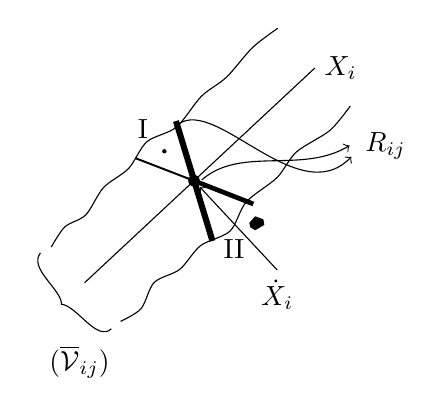
\begin{tikzpicture}[x=1cm,y=1cm,rotate=43]
\draw (0,0)--(4,0) node[right] {$X_i$};
\draw plot[smooth] coordinates {(0,.62)(.3,.69)(.6,.62)(1,.72)(1.4,.68)(1.8,.77)(2.2,.65)(2.7,.72)(3.1,.68)(3.6,.73)(4,.69)};
\draw plot[smooth] coordinates {(0,-.67)(.3,-.73)(.65,-.6)(1,-.7)(1.4,-.66)(1.8,-.78)(2.2,-.65)(2.7,-.69)(3.1,-.62)(3.6,-.71)(4,-.66)};
\draw[line width=.7pt] (1.55,.72)--(1.9,0);
\draw[line width=1.7pt] (1.9,0)--(2.25,-.73);
\draw[line width=2.2pt] (1.55,-.72)--(2.25,.71);
\fill (1.9,0) circle (2.1pt);
\fill (1.88,.53) circle (.8pt);
\fill (2.05,-.87)--(2.16,-.86)--(2.21,-.96)--(2.17,-1.02)--(2.04,-.99)--(2.02,-.92)--cycle;
\node at (1.87,.92) {$\mathrm I$};
\node at (1.68,-.98) {$\mathrm{II}$};
\draw[->] (1.9,-1.55)--(1.9,-.11);
\node[below] at (1.9,-1.55) {$\dot X_i$};
\draw[->] (2.18,.66) .. controls (2.85,.72) and (2.58,-1.20) .. (3.57,-1.14);
\draw[->] (1.98,-.06) .. controls (2.64,-.08) and (2.96,-.88) .. (3.65,-1.02);
\node[right] at (3.7,-1.08) {$R_{ij}$};
\draw (-.15,-.66) .. controls (-.4,-.66) and (-.27,-.15) .. (-.4,0) .. controls (-.27,.14) and (-.4,.62) .. (-.15,.66);
\node[below left] at (-.14,-.8) {$(\unsure{\overline{\mathcal V}_{ij}})$};
\end{tikzpicture}}
où dans $\mathcal V_{ij}^*$ il y a des morceaux suppl. ``idiots'' I et II \ldots}
\margin{58}
